\documentclass{article}
\usepackage{amsmath}
\usepackage{amssymb}
\usepackage{graphicx}

\begin{document}

\title{4D Euclidean Space Visualization}
\author{Jonah Schwartzman}
\date{\today}

\maketitle

\section{Introduction}
Our goal is to visualize 4D Euclidean space on a 2D screen.
\newline\newline We will attempt a projection from 4D space to 2D space.
\newline\newline User can translate and rotate the 2D frame around in 4D space.
\newline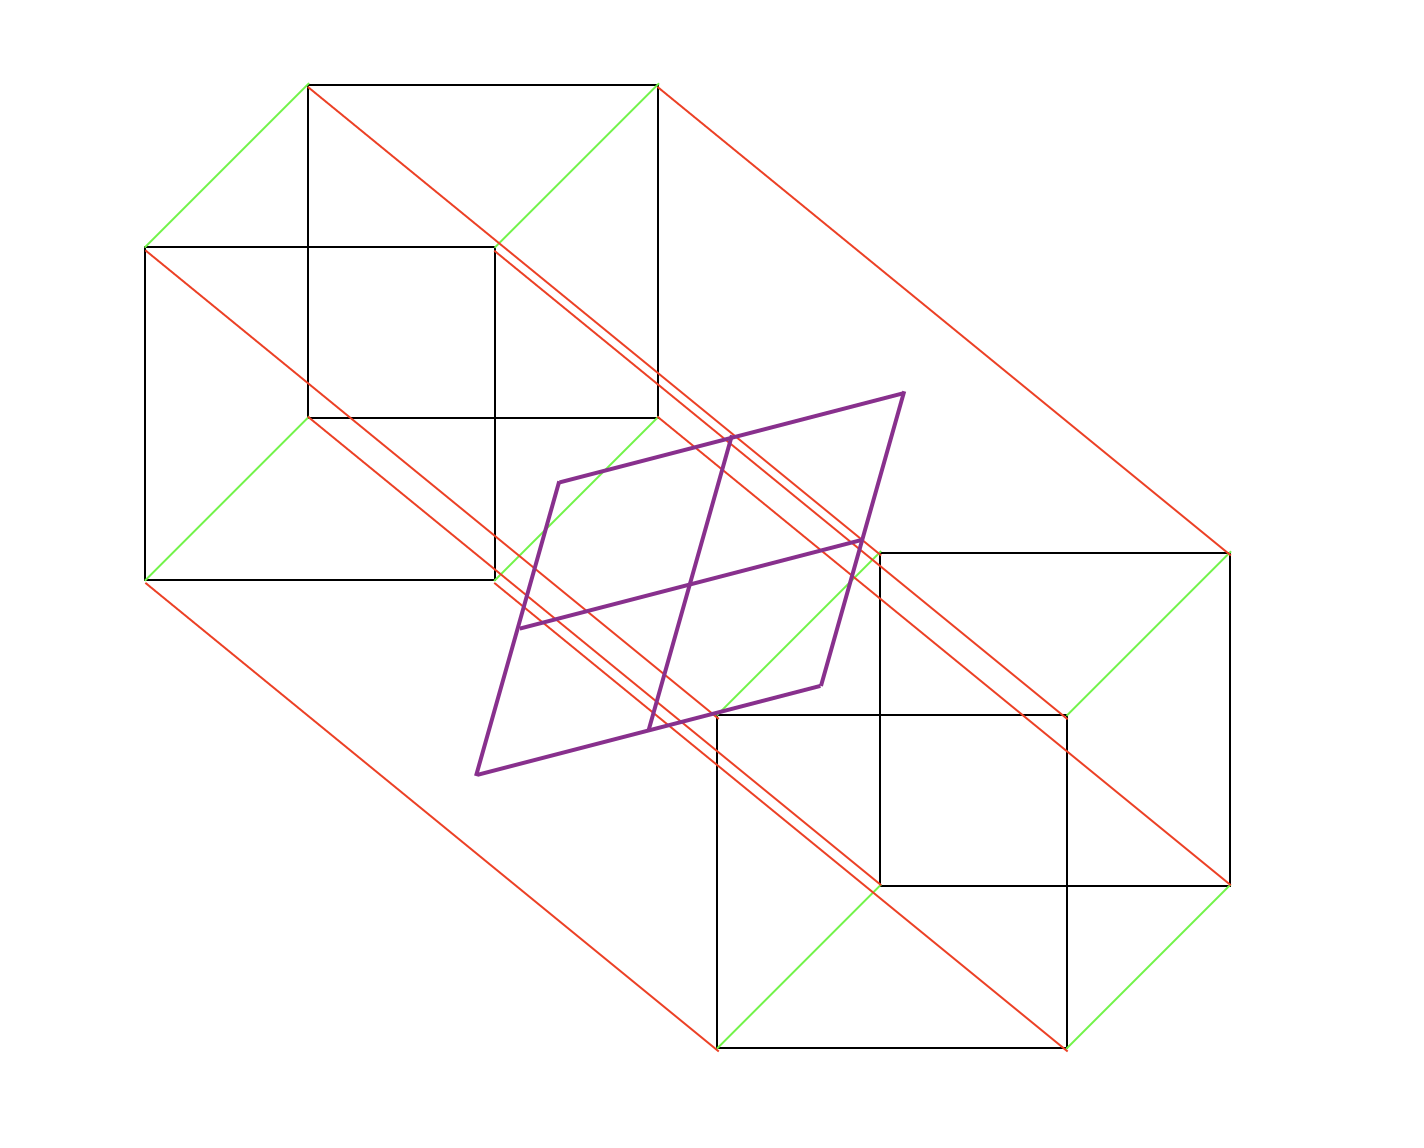
\includegraphics[scale=0.5]{4dProjection.png}
\newline In this diagram, the black squares represent the x and y axis, the green lines represent the z axis, and the red lines represent the w axis.
\newline The purple frame represents the view screen somewhere in 4d space.

\section{Transformations and Projections}
\subsection{The goal}
At a high level this transformation from 4d space to 2d space can be thought of as a function:
\[T: \mathbb{R}^4 \to \mathbb{R}^2\]
which can be represented as a 2x4 matrix $A$ in the equation
\[A\begin{pmatrix}
x \\ y \\ z \\ w
\end{pmatrix} = T\left(\begin{pmatrix}
    x \\ y \\ z \\ w
    \end{pmatrix}\right) = \begin{pmatrix}
X \\ Y
\end{pmatrix}\]
\subsection{Finding a good T}

If $T = \begin{pmatrix}
    1 & 0 & 0 & 0 \\
    0 & 1 & 0 & 0
\end{pmatrix}$, then $T\begin{pmatrix}
    x \\ y \\ z \\ w
    \end{pmatrix} = \begin{pmatrix}
    x \\ y
    \end{pmatrix}$,
so $T$ is a projection onto the x-y plane.
\newline\newline Generally, If $T = \begin{pmatrix}
    1_i \\
    1_j
\end{pmatrix}$, then $Tv = \begin{pmatrix}
    v_i \\ v_j
    \end{pmatrix}$,
so $T$ is a projection onto the $v_i$-$v_j$ plane.
\newline\newline We want a way to rotate from a projection onto one plane to another.
\newline\newline Let $R_{ij} \in\mathbb{R}^{2\times4}=$
\[\begin{pmatrix}
    \cos(\theta)_i & -\sin(\theta)_j \\
    \sin(\theta)_i & \cos(\theta)_j
\end{pmatrix}\]
So $R_{yw} \in\mathbb{R}^{2\times4}=$
\[\begin{pmatrix}
    0 & \cos(\theta)_i & 0 & -\sin(\theta)_j \\
    0 & \sin(\theta)_i & 0 & \cos(\theta)_j
\end{pmatrix}\]
Notice that $2\times4$ matrices cannot be chained together, we could have a situation like:
\[\begin{pmatrix}
    &\\&\\&\\
\end{pmatrix}\begin{pmatrix}
    & & &
\end{pmatrix}
\begin{pmatrix}
    &\\&\\&\\
\end{pmatrix}\begin{pmatrix}
    & & &
\end{pmatrix}
\begin{pmatrix}
    &\\&\\&\\
\end{pmatrix}\begin{pmatrix}
    & & &
\end{pmatrix}\]
with these matrices, $\mathbb{R}^{2}\to\mathbb{R}^2$ or $\mathbb{R}^{4}\to\mathbb{R}^4$
\newline There are now 6 planes to rotate between
\newline $\theta, \alpha, \beta, \gamma, \phi, \psi$
\newline Imagine
\[T(\frac{1}{6}(\begin{pmatrix}
    \cos(\theta) & -\sin(\theta) & 0 & 0 \\
    \sin(\theta) & \cos(\theta) & 0 & 0 \\
    0 & 0 & 1 & 0 \\
    0 & 0 & 0 & 1

\end{pmatrix}+
\begin{pmatrix}
    \cos(\alpha) & 0 & -\sin(\alpha) & 0 \\
    0 & 1 & 0 & 0 \\
    \sin(\alpha) & 0 & \cos(\alpha) & 0 \\
    0 & 0 & 0 & 1
\end{pmatrix}+
\begin{pmatrix}
    \cos(\beta) & 0 & 0 & -\sin(\beta)\\
    0 & 1 & 0 & 0 \\
    0 & 0 & 1 & 0 \\
    \sin(\beta) & 0 & 0 & \cos(\beta)
\end{pmatrix}+\]
\newline
\[\begin{pmatrix}
    1 & 0 & 0 & 0 \\
    0 & \cos(\gamma) & -\sin(\gamma) & 0 \\
    0 & \sin(\gamma) & \cos(\gamma) & 0 \\
    0 & 0 & 0 & 1
\end{pmatrix}+
\begin{pmatrix}
    1 & 0 & 0 & 0 \\
    0 & \cos(\phi) & 0 & -\sin(\phi) \\
    0 & 0 & 1 & 0 \\
    0 & \sin(\phi) & 0 & \cos(\phi)
\end{pmatrix}+
\begin{pmatrix}
    1 & 0 & 0 & 0 \\
    0 & 1 & 0 & 0 \\
    0 & 0 & \cos(\psi) & -\sin(\psi) \\
    0 & 0 & \sin(\psi) & \cos(\psi)
\end{pmatrix}
))\]
with $T$
\[=\begin{pmatrix}
    1 & 1 & 1 & 1 \\
    1 & 1 & 1 & 1
\end{pmatrix}\]


\end{document}